\newif \ifhandout \handoutfalse
\newif \ifbackup \backuptrue

% \handouttrue

\documentclass[a4paper, 12pt, aspectratio=169,
\ifhandout handout \else \fi
]{beamer}
\usetheme{Pittsburgh}
\usecolortheme{whale}
\usefonttheme{structurebold}

% \definecolor{green}{rgb}{0.5,0.5,0.5}

\RequirePackage{listings}
\lstset{
    % backgroundcolor=\color{green},
    basicstyle=\ttfamily,
    language=bash,
    keywordstyle=\bf\ttfamily,
    keepspaces=true,
    showstringspaces=false,
    columns=flexible,
    keywords=git,
}

\usepackage{mdframed}

\usepackage{combelow}

\mode<presentation>
\setbeamertemplate{footline}[frame number]
\setbeamertemplate{frametitle}[default][center]
\beamertemplatenavigationsymbolsempty

\usepackage{tikz}
\usepackage[outline]{contour}
\contourlength{1.2pt}

\usepackage{xcolor}
\usepackage{color}
% \usepackage{tcolorbox}
% \newcommand{\red}[1]{{\color{red}{#1}}}
% \newcommand{\green}[1]{{\color{dkgreen}{#1}}}
% \newcommand{\white}[1]{{\color{white}{#1}}}
% \newcommand{\blue}[1]{{\color{blue}{#1}}}

% \newcommand{\highlight}[2]{%
%                   \colorbox{#1}{$\displaystyle#2$}}
% \newcommand{\highlightb}[2]{%
%                   \fcolorbox{#1}{white}{$\displaystyle#2$}}
% \def\Put(#1,#2)#3{\leavevmode\makebox(0,0){\put(#1,#2){#3}}}

\begin{document}
\title{Introducción a git}
% \author{Guido Martínez}
\date{}

\begin{frame}
    \titlepage
\end{frame}

\newcommand{\backupbegin}{
   \newcounter{finalframe}
   \setcounter{finalframe}{\value{framenumber}}
}
\newcommand{\backupend}{
   \setcounter{framenumber}{\value{finalframe}}
}

\begin{frame}
    \frametitle{¿Qué es?}
    \begin{itemize}
        \item Sistema de control de versiones (SCM).
            \pause

        \item Esencialmente, rastrea los cambios de nuestros archivos
            (generalmente código fuente), y permite ir hacia atrás si hace falta.
            \pause

        \item Creado por Linus Torvalds en 2005...  \pause en semanas.
    \end{itemize}
    \pause

    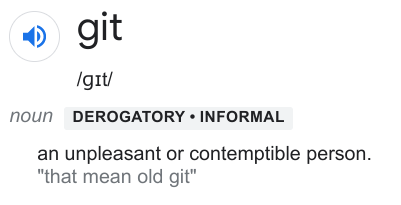
\includegraphics[scale=0.5]{defn.png}
\end{frame}

\begin{frame}
    \frametitle{¡Ah! ¿Como SVN?}
    \begin{itemize}
        \item \textbf{No.} \pause
            Si conocen SVN/CVS, les conviene olvidar todo lo que saben.

            \pause
        \item Principal diferencia: \emph{distribuido}.
    \begin{mdframed}[
            linecolor=black,
            outerlinewidth=0,
            innertopmargin=10,
            innerbottommargin=10,
            leftmargin=1,
            rightmargin=1,
            roundcorner=1pt
            ]
        \begin{center}
            Cada desarrollador tiene \emph{todo} el código
            y \emph{toda} la historia.
        \end{center}
    \end{mdframed}
    \pause

    \item Enviar/recibir cambios de otro host es \emph{infrecuente}.
        Incluso sin ningún otro colaborador, \texttt{git} ayuda para organizarse.
    \end{itemize}
\end{frame}

\begin{frame}[fragile]
    \frametitle{Flexible, jerárquico, distribuido}
    \begin{center}
    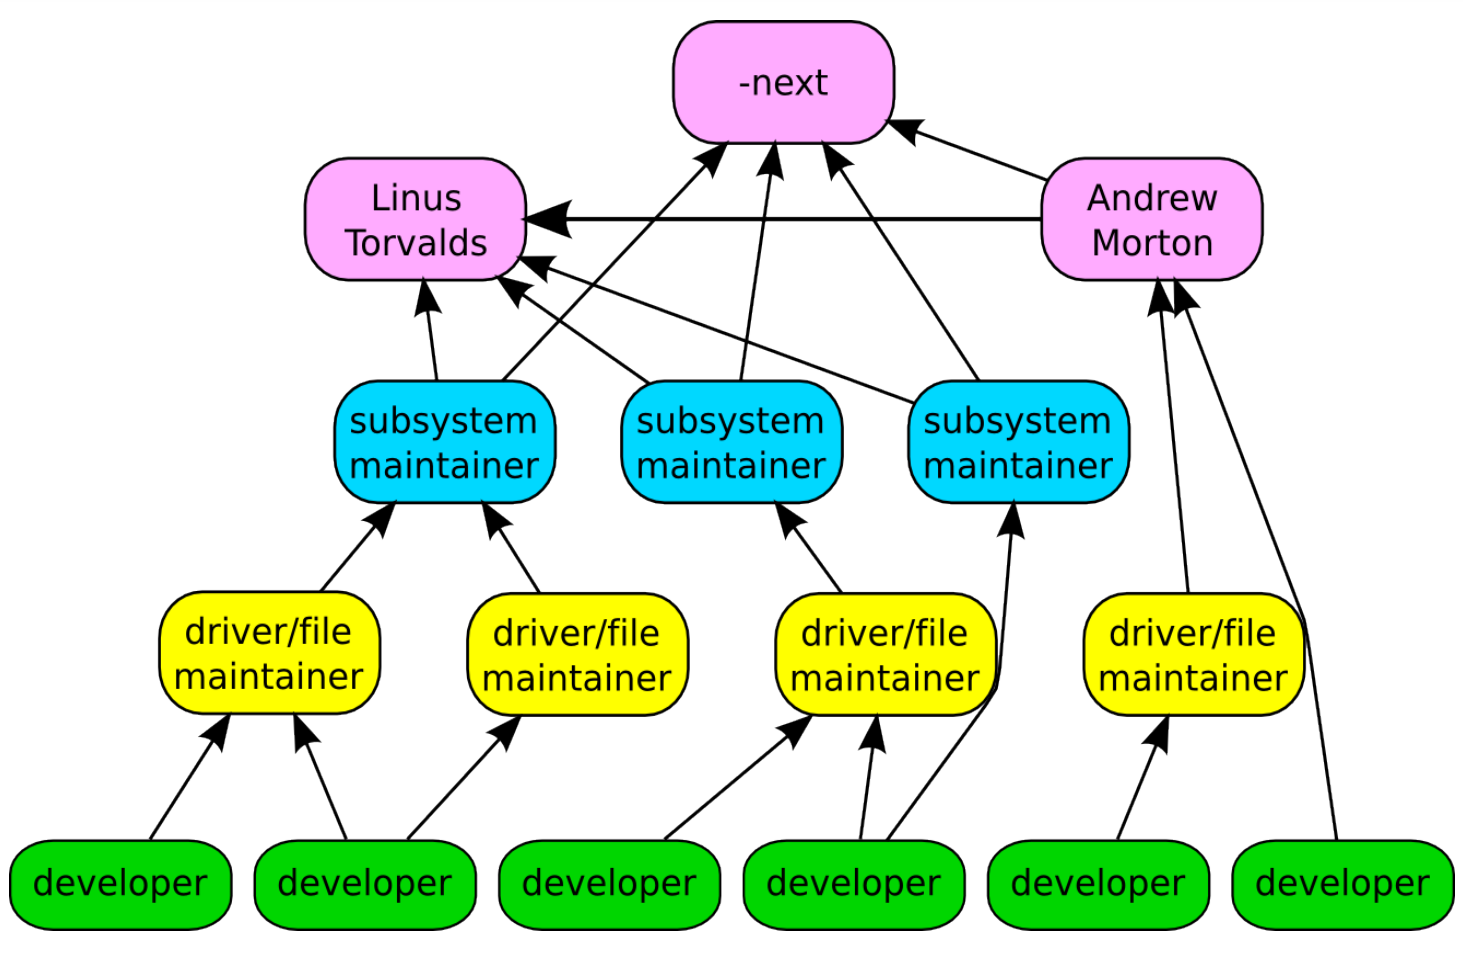
\includegraphics[keepaspectratio, height=0.8\textheight, width=\linewidth]{flow.png}
    \end{center}
\end{frame}

\begin{frame}[fragile]
    \frametitle{Génesis}
    ¿Cómo arranca un repositorio?
    \begin{onlyenv}<1>
        \begin{itemize}
            \item 1, desde cero:
\begin{lstlisting}
~$ mkdir proyecto/
~$ cd proyecto/
~/proyecto$ git init
Initialized empty Git repository in /home/guido/proyecto/.git/
\end{lstlisting}
        \end{itemize}
    \end{onlyenv}
    \begin{onlyenv}<2>
        \begin{itemize}
            \item 2, clonando:
                \begin{lstlisting}[basicstyle=\ttfamily\small]
~$ git clone https://github.com/torvalds/linux
Cloning into 'linux'
remote: Enumerating objects: 8716629, done.
remote: Total 8716629 (delta 0), [...]
Receiving objects: 100% [...]
Resolving deltas: 100% [...]
Updating files: 100% [...], done.
~$
\end{lstlisting}
        \end{itemize}
    \end{onlyenv}
\end{frame}

\begin{frame}[fragile]
    \frametitle{Mirando el estado...}
    \begin{onlyenv}<1>
    \begin{lstlisting}
~/proyecto$ git status
On branch master

No commits yet

nothing to commit (create/copy files and use "git add" to track)
    \end{lstlisting}
    \end{onlyenv}
    \begin{onlyenv}<2>
    \begin{lstlisting}
~/proyecto$ touch blah.c
~/proyecto$ echo 'int main(){return 0;}' > main.c
~/proyecto$ git status
On branch master

No commits yet

Untracked files:
  (use "git add <file>..." to include in what will be committed)
        blah.c
        main.c

nothing added to commit but untracked files present
     (use "git add" to track)
    \end{lstlisting}
    \end{onlyenv}
\end{frame}

\begin{frame}[fragile]
    \frametitle{Estados}
    \begin{center}
    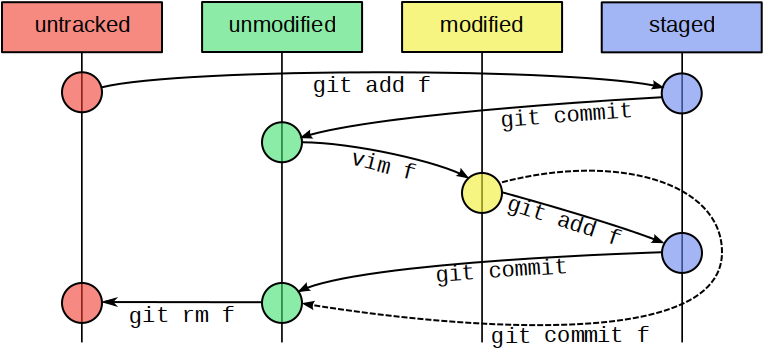
\includegraphics[keepaspectratio, height=0.8\textheight, width=\linewidth]{estados.png}
    \end{center}
\end{frame}

\begin{frame}[fragile]
    \frametitle{Staging area}
\begin{lstlisting}
~/proyecto$ git add main.c
~/proyecto$ git status
On branch master

No commits yet

Changes to be committed:
  (use "git rm --cached <file>..." to unstage)
        new file:   main.c

Untracked files:
  (use "git add <file>..." to include in what will be committed)
        blah.c
\end{lstlisting}
\end{frame}


    % \begin{itemize}
    %     \item No trackeado
    %     \item Trackeado, sin cambios
    %     \item Trackeado, con cambios
    % \end{itemize}

\begin{frame}[fragile]
    \frametitle{Commit}
\begin{lstlisting}
~/proyecto$ git commit -m "Inicio proyecto"
[master (root-commit) 5a2e447] Inicio proyecto
 1 file changed, 1 insertions(+), 0 deletions(-)
 create mode 100644 main.c
\end{lstlisting}\pause
\begin{lstlisting}
~/proyecto$ git status
On branch master
Untracked files:
  (use "git add <file>..." to include in what will be committed)
        blah.c

nothing added to commit but untracked files present (use "git add" to track)
\end{lstlisting}
\end{frame}

\begin{frame}[fragile]
    \frametitle{¿Qué es un commit?}
    \begin{itemize}
        \item Snapshot \textbf{completa} del árbol (con optimizaciones de espacio)
        \item Es un hash \textbf{criptográfico} de:
        \begin{itemize}
            \item Todos los archivos
            \item Mensaje de commit
            \item Autor, fecha, etc
            \item Commit padre
        \end{itemize}
        \pause
    \item Criptográfico = no se puede invertir, ni encontrar colisiones (eficientemente)
        \pause
    \item Obviamente... con optimizaciones para no recomputar el hash desde cero
        cada vez (ver \emph{Merkle trees})
    \end{itemize}
\end{frame}

\begin{frame}[fragile]
    \frametitle{Log}
    \begin{onlyenv}<1>
        \begin{lstlisting}
~/proyecto$ git log
commit 4e80d6ce4a584e0a1d0708489f29dd60f6d67758
Author: Guido Martínez <mtzguido@gmail.com>
Date:   Tue Apr 19 10:01:43 2022 -0300

    Inicio proyecto
        \end{lstlisting}
    \end{onlyenv}
    \begin{onlyenv}<2>
        \begin{lstlisting}
~/proyecto$ git log --stat
commit 4e80d6ce4a584e0a1d0708489f29dd60f6d67758
Author: Guido Martínez <mtzguido@gmail.com>
Date:   Tue Apr 19 10:01:43 2022 -0300

    Inicio proyecto

 main.c | 1 +
 1 file changed, 1 insertion(+)
        \end{lstlisting}
    \end{onlyenv}
    \begin{onlyenv}<3>
        \begin{lstlisting}
~/proyecto$ git log -p
commit 4e80d6ce4a584e0a1d0708489f29dd60f6d67758
Author: Guido Martínez <mtzguido@gmail.com>
Date:   Tue Apr 19 10:01:43 2022 -0300

    Inicio proyecto

diff --git a/main.c b/main.c
new file mode 100644
index 0000000..2c99a52
--- /dev/null
+++ b/main.c
@@ -0,0 +1 @@
+int main(){return 0;}
        \end{lstlisting}
    \end{onlyenv}
\end{frame}

\begin{frame}[fragile]
    \frametitle{Diff Unificado}
    \begin{lstlisting}[basicstyle=\ttfamily\footnotesize]
~/proyecto$ git show
commit 61af2d85a1c4d2279c0dc6bc514accb1d96484df
Author: Guido Martínez <mtzguido@gmail.com>
Date:   Tue Apr 19 10:20:24 2022 -0300

    Corregir typo

diff --git a/main.c b/main.c
index 7c0913d..00dd468 100644
--- a/main.c
+++ b/main.c
@@ -1,5 +1,5 @@
 int main()
 {
-       printf("Holamundo\n");
+       printf("Hola mundo\n");
        return 0;
 }
\end{lstlisting}
\end{frame}

\begin{frame}
    \frametitle{Digresión: buenas prácticas}
    \begin{itemize}
        \item Commits lo más pequeños posibles (``atómicos''): permite revertir fácilmente
        \item Mensajes descriptivos: ``cambios'' vs ``Corregir algoritmo de Peterson con mfence''
        \item Nunca romper el build: permite bisectar (\texttt{git bisect})
    \end{itemize}
\end{frame}

\begin{frame}[fragile]
    \frametitle{Borrar archivos}
    \begin{itemize}
        \item \lstinline`git rm` borra un archivo (y anota el cambio
            en la staging area). Es lo mismo que hacer \lstinline`rm` y
            \lstinline`git add`.
    \end{itemize}
\begin{lstlisting}[basicstyle=\ttfamily\footnotesize]
~/proyecto$ git rm main.c
rm 'main.c'
~/proyecto$ git status
On branch master
Your branch is up to date with 'origin/master'.

Changes to be committed:
  (use "git restore --staged <file>..." to unstage)
        deleted:    main.c
$ git commit -m "Borrar main"
[master f068e5f] Borrar main
 1 file changed, 5 deletions(-)
 delete mode 100644 main.c
\end{lstlisting}
\end{frame}

\begin{frame}[fragile]
    \frametitle{Config}
    \begin{lstlisting}
$ git config --global user.name "Alan Turing"
$ git config --global user.email "aturing@princeton.edu"
    \end{lstlisting}
\end{frame}

\begin{frame}[fragile]
    \frametitle{Remotes}
    Hasta ahora, \textbf{nada} requirió de la red.
    \pause
            \begin{minipage}[t][8cm]{\textwidth}
    \begin{onlyenv}<2>
    \begin{center}
    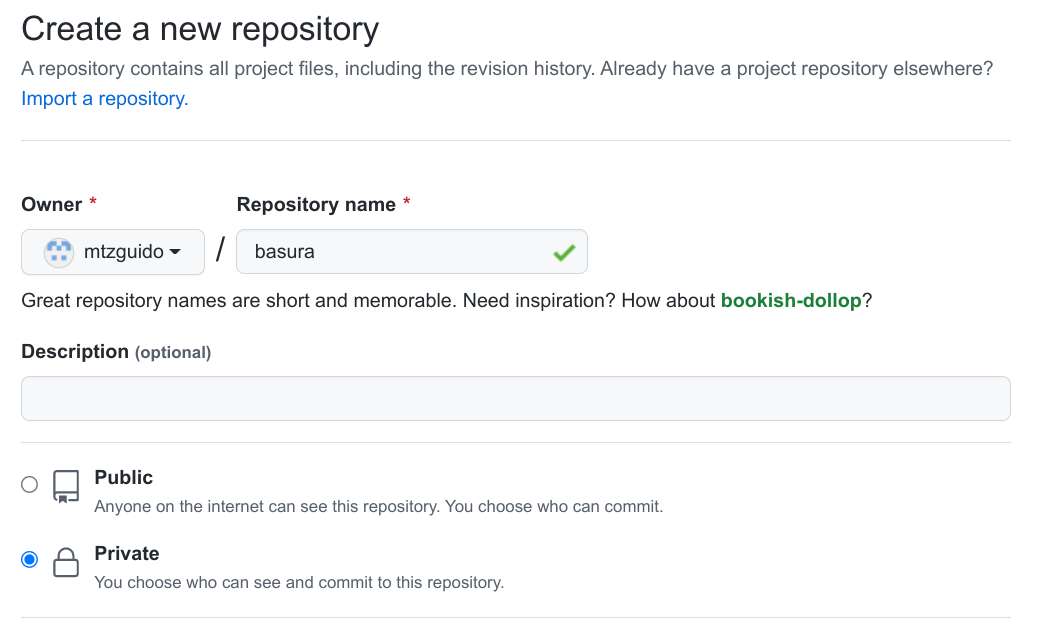
\includegraphics[keepaspectratio, height=0.8\textheight, width=\linewidth]{basura.png}
    \end{center}
    \end{onlyenv}
    \begin{lstlisting}[basicstyle=\ttfamily\footnotesize]
~/proyecto$ git remote add origin git@github.com:mtzguido/basura
~/proyecto$ git push -u origin master
Enumerating objects: 9, done.
Counting objects: 100% (9/9), done.
Delta compression using up to 4 threads
Compressing objects: 100% (5/5), done.
Writing objects: 100% (9/9), 789 bytes | 789.00 KiB/s, done.
Total 9 (delta 0), reused 0 (delta 0), pack-reused 0
To github.com:mtzguido/basura
 * [new branch]      master -> master
branch 'master' set up to track 'origin/master'.
~/proyecto$
    \end{lstlisting}
    \begin{onlyenv}<3>
    \end{onlyenv}
            \end{minipage}
\end{frame}

\begin{frame}
    \frametitle{Push/pull}
    \begin{itemize}
        \item \textbf{Push:} actualiza el repo remoto desde el local (sólo cambios commiteados)
        \item \textbf{Pull:} actualiza el repo local desde el remote
    \end{itemize}
\end{frame}

\begin{frame}[fragile]
    \begin{center}
        \Huge \bf La base está...
    \end{center}
\end{frame}

\begin{frame}[fragile]
    \frametitle{Revirtiendo cambios}
    \begin{itemize}
        \item \lstinline`git checkout <file>`: revierte cambios locales.
        \item \lstinline`git reset`: vacía el staging area.
        \item \lstinline`git reset <commit>`: vuelve al commit, sin modificar archivos.
        \item \lstinline`git reset --hard <commit>`: vuelve al commit, descartando
            \textbf{todo}.
    \end{itemize}
\end{frame}

\begin{frame}
    \frametitle{Branches}
    \begin{itemize}
        % \item Concepto de branch en SVN: otra carpeta...
        \item Un branch es un nombre que ``apunta'' o ``sigue'' a un commit hash
        \item \lstinline`git branch featureX`: crear y moverse a un branch
        \item \lstinline`git checkout <b>`: cambiar de branch
        \item \lstinline`master` suele ser la rama principal
    \end{itemize}
\end{frame}

\begin{frame}
    \frametitle{Merges}
    \begin{itemize}
        \item Toma dos commits y \emph{une} sus cambios en uno.
        \item En branch \emph{source} \lstinline`git merge <commit>`. Pull tiene merge implícito, push sólo permite ``fast-forwards''.
    \end{itemize}
    \pause
    \begin{minipage}[t][4cm]{\textwidth}
    \begin{center}
        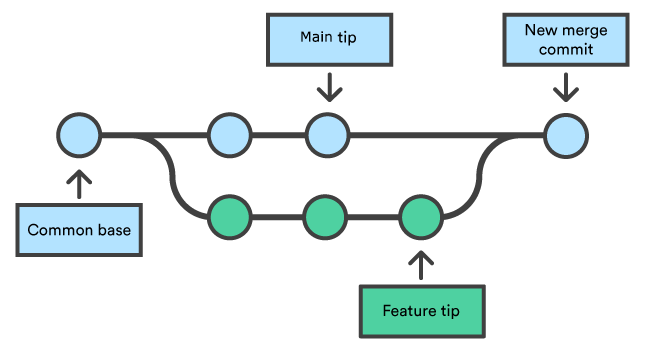
\includegraphics[keepaspectratio, height=0.5\textheight, width=\linewidth]{mergeasd.png}
    %     \begin{onlyenv}<2>
    %         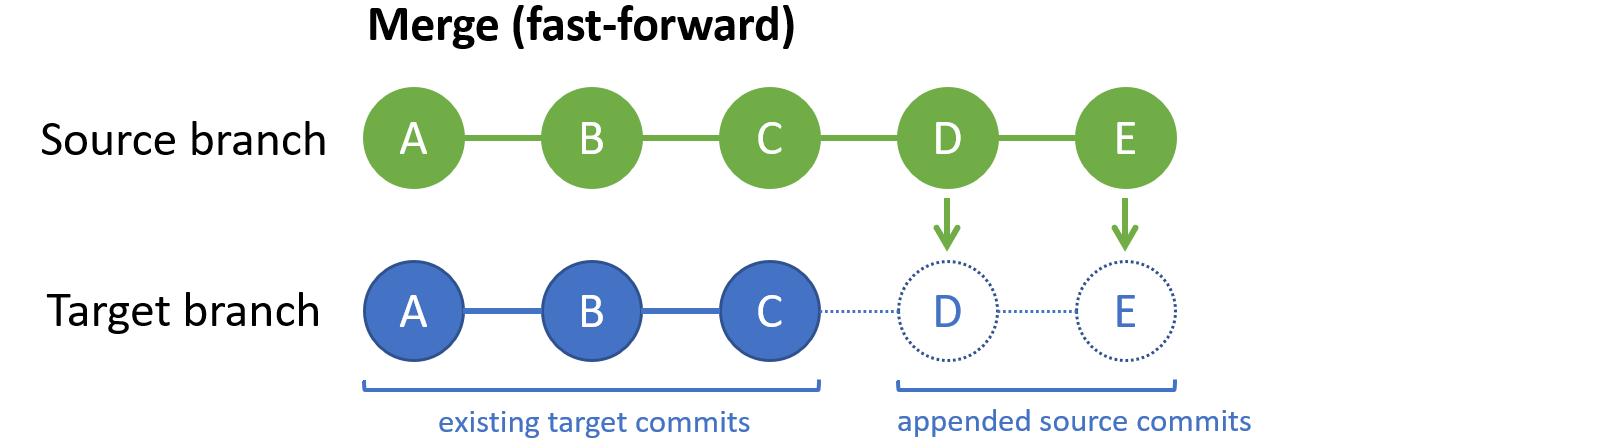
\includegraphics[keepaspectratio, height=0.6\textheight, width=\linewidth]{merge1.png}
    %     \end{onlyenv}
    %     \begin{onlyenv}<3>
    %         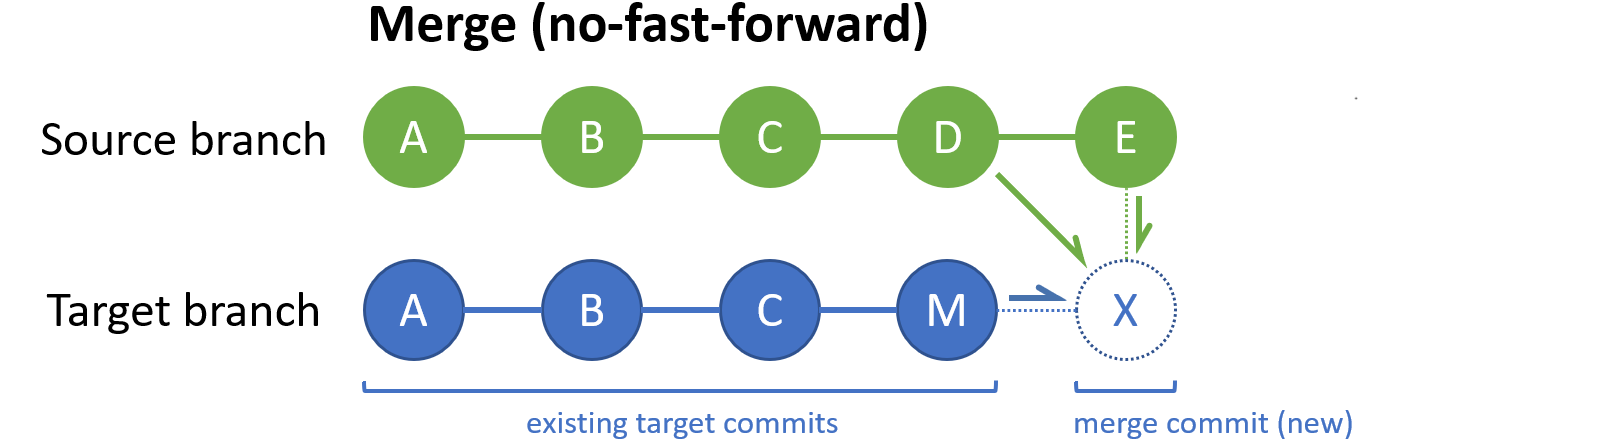
\includegraphics[keepaspectratio, height=0.6\textheight, width=\linewidth]{merge2.png}
    %     \end{onlyenv}
    \end{center}
    \end{minipage}
    \pause
    \begin{itemize}
        \item Posiblemente haya que \textbf{corregir conflictos}
        \item Interfaz gráfica: \texttt{gitg} (o \lstinline`git log --graph`)
    \end{itemize}
\end{frame}

\begin{frame}
    \frametitle{Rebase}
    \begin{itemize}
        \item Similar a un merge... pero ``reescribe la historia''
            \begin{minipage}[t][4cm]{\textwidth}
                \begin{center}
                    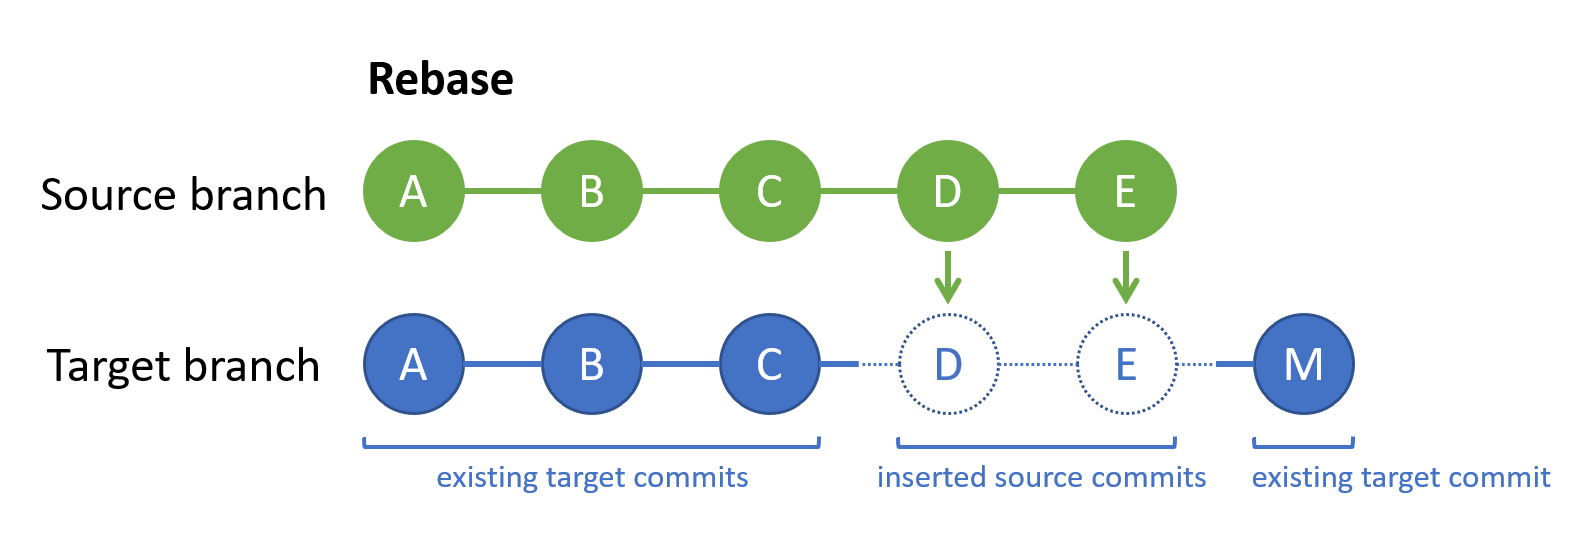
\includegraphics[keepaspectratio, height=0.5\textheight, width=\linewidth]{merge3.png}
                \end{center}
            \end{minipage}
        \item Generalmente sólo se hace en ramas privadas
    \end{itemize}
\end{frame}

\begin{frame}[fragile]
    \frametitle{Clean}
    Usar con cuidado...
    \begin{itemize}
        \item \lstinline`git clean -dfx`: borra todo lo que no esté trackeado/staged
        \item \lstinline`git clean -x`: borra sólo archivos ignorados (suele ser seguro)
        \item Flag \texttt{-n}: no hacer nada, imprimir lo que haría
    \end{itemize}
\end{frame}

\begin{frame}[fragile]
    \frametitle{Otras features}
    \begin{itemize}
        \item Aliases: abreviar comandos (\lstinline`git st` == \lstinline`git status`, etc).
        \item Hooks: el remoto toma alguna acción al recibir un push.
        \item ``Plomería'' vs ``Porcelana'', permite scripting.
        \item \lstinline`git bisect`: encontrar el commit que introdujo un bug.
        \item \lstinline`git worktree`: mismo repositorio, $N$ árboles de trabajo.
        \item \lstinline`git bisect` automático.
        \item \lstinline`git blame`: ver quién escribió cada línea.
    \end{itemize}
\end{frame}

\begin{frame}[fragile]
    \frametitle{Referencias}
    \begin{itemize}

        \item Libro:\\
            \url{https://git-scm.com/book}

        \item TryGit:\\
            \url{https://try.github.io/}

        \item A Visual Git Reference:\\
            \url{https://marklodato.github.io/visual-git-guide/index-en.html}

        \item Git From the Bottom Up:\\
            \url{http://ftp.newartisans.com/pub/git.from.bottom.up.pdf}

        \item Why Git is Better than X:\\
            \url{https://bryankaraffa.github.io/whygitisbetter/}

        \item Learn Git Branching: \\
            \url{https://learngitbranching.js.org/}

        \item Charla Torvalds:\\
            \url{https://www.youtube.com/watch?v=4XpnKHJAok8}
    \end{itemize}
\end{frame}

\end{document}
